% !TEX root = ../main.tex

\chapter{绪论}

\section{研究背景和意义}

医疗图像分割技术是计算机视觉和模式识别技术应用在诸如X-Ray CT(X光计算机断层扫描成像)、MRI(磁共振成像)和Ultrasound(超声成像)等医疗图像上,
针对特定的目标,譬如肺部动脉/静脉血管、乳腺肿块,肺癌结节,进行逐体素(Voxel)的分类。本文聚焦肺部CT扫描图像,研究肺部支气管树状结构的气道分割提取技术。


肺部和呼吸系统疾病对人体健康威胁巨大,自2019年底、2020年初爆发的全球性新冠肺炎COVID-19疫情严重冲击人类的公共卫生与生命健康。三年多来,世界各国在抗击新冠肺炎疫情方面付出了惨重的生命代价和社会经济损失。新型冠状病毒经由空气为媒介传播,通过呼吸道进入肺部并感染细胞。包括肺癌在内的一些肺部疾病,慢性
阻塞性肺疾病(COPD)\cite{fetita2004pulmonary}、急性呼吸窘迫综合症\cite{howling1998significance}、闭塞性细支气管炎\cite{shaw2002role}、特发性肺纤维化\cite{wu2019computed}、肺挫伤\cite{li2019application}等导致肺支气管气道树的形态学变化。
支气管气道树的形态学三维模型通过从基于CT扫描的肺部图像中精确分割出来,是分析包括哮喘、支气管扩张和肺气肿在内的肺部疾病的关键步骤。测量精确分割出来的支气管的气道管腔
尺寸和管壁厚度,可以用于辅助诊断肺栓塞\cite{estepar2013computed}, 揭示慢性阻塞性肺部疾病COPD患者的异常病症。除了上述这些疾病诊断治疗之外,本文研究肺部支气管气道
树分割的一个直接动因是为了开发支气管镜和支气管导航与活体检测的手术机器人。手术机器人驱动细长柔性的支气管镜器械,伸入支气管,沿着气道导航至疑似(肺部)病灶部位,对
病灶处细胞进行活体采样返回,进而化验诊断出疾病。本文作者所在的工作单位就在开发国产的支气管镜导航/检测的手术机器人,而支气管气道树的精确分割就是非常重要的前置研发步骤。
构建出支气管气道树的分割模型后,输入患者的肺部CT扫描图像数据,就可以输出包含精确的三维空间信息的支气管气道树结构。将这个支气管气道树的结构模型“喂给”支气管镜导航机器人
(Bronchoscopy and endobronchical navigation robot),在医生的监视与操纵下,机器人就可以被引导进入支气管管腔内,进行疾病的诊断与治疗了。

{\heiti 支气管气道树的分支结构。} 本文研究支气管气道树的分割,有必要先了解一下支气管数状结构的气道解剖结构。从图\ref{fig:branches_of_bronchial_tree}中可以看出,支气管气道树的分支结构非常复杂,从气管(Trachea)往下分为左、右两支主支气管(Main bronchus),左右两支主支气管各自分岔为上叶支气管(Superior lobar bronchus)、中叶支气管(Middle lobar bronchus)和下叶支气管(Inferior
 lobar bronchus)。在每个肺叶内,起于肺叶的支气管继续分岔为多个肺段支气管(Segmental bronchi)。肺段支气管最后分为更细小的支气管到达肺泡。

\begin{figure}[!htp]
	\centering
	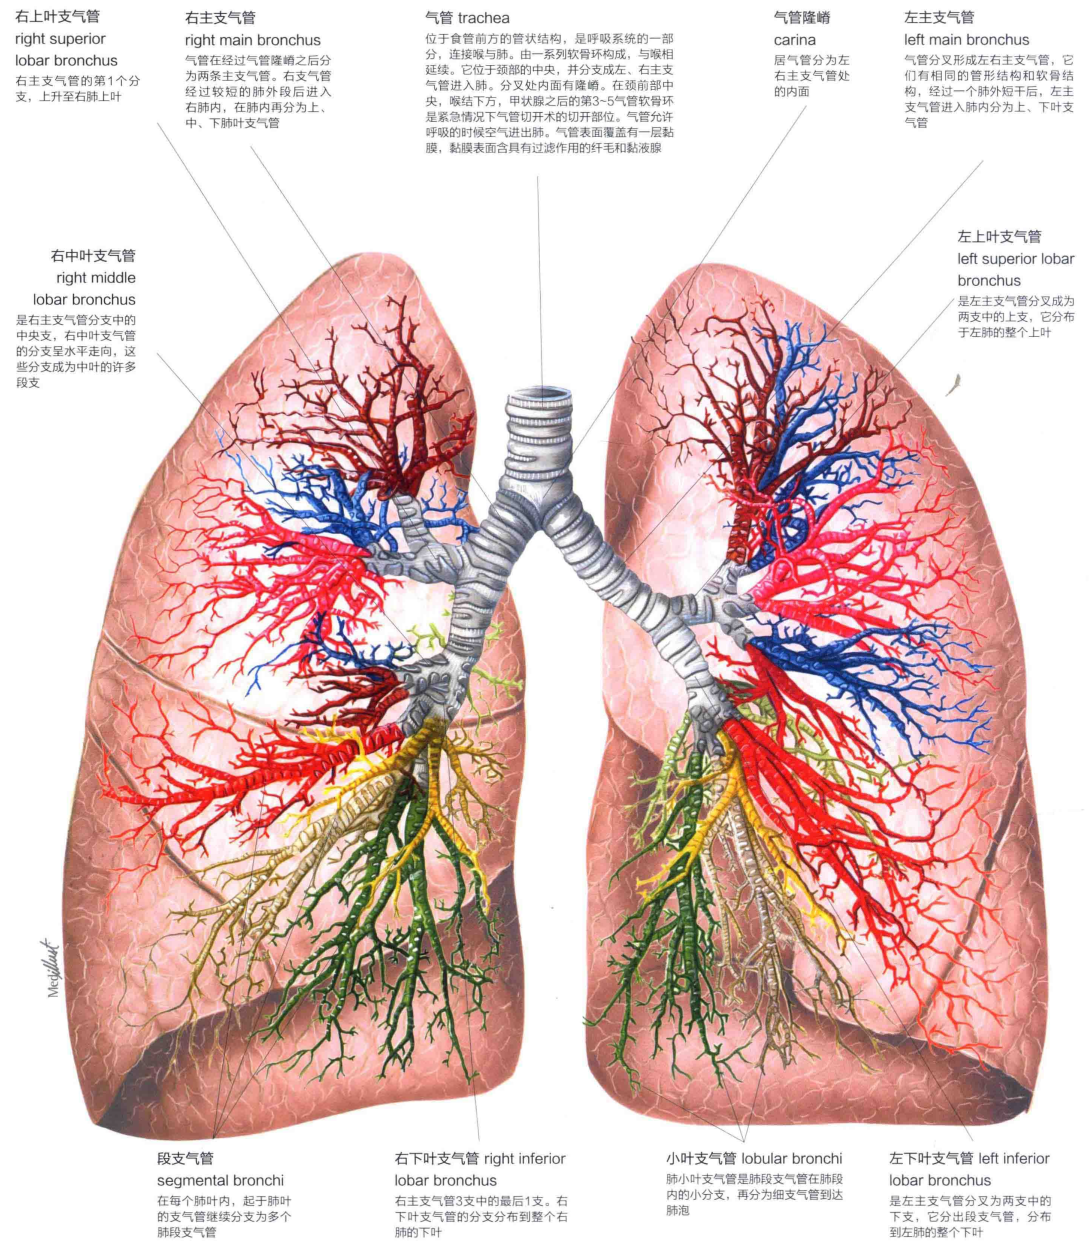
\includegraphics[width=0.9 \textwidth]{branches_of_the_bronchial_tree}
	\bicaption[肺部支气管气道树的分支结构]
		{肺部支气管气道树的分支结构\parencite{humananatomy2nd}}
		{The branch structure of pulmonary bronchial airway tree}
	\label{fig:branches_of_bronchial_tree}	
\end{figure}

如此繁复,从粗到细不断分化,面对如此稠密细小的支气管气道树,进行分割前需要经验丰富的临床专家进行非常细粒度的标注。手工标注耗费大量时间,
成本高昂且支气管越细小,标注越困难,易于出错。 标注任务艰巨繁重,急需开发新的算法或模型来帮助临床医生解决支气管气道树分割的问题。

\section{本研究的应用前景}

肺部支气管气道树的自动化分割是呼吸系统肺部疾病诊断治疗的一个重要问题和研究领域,在实际应用中具有非常重要的作用,提高医疗技术水平。当前,在
作者所在的医疗机器人行业,本研究项目有如下的应用前景:
\begin{itemize}
	\item {\heiti 导管手术机器人 }
	由于肺部支气管气道树三维模型具有精确的空间位置信息,CT扫描建立的坐标系赋予DICOM医疗图像每个像素都有相应的坐标位置信息,如图\ref{fig:coordinate}所示。
	\begin{figure}[!htp]
		\centering
		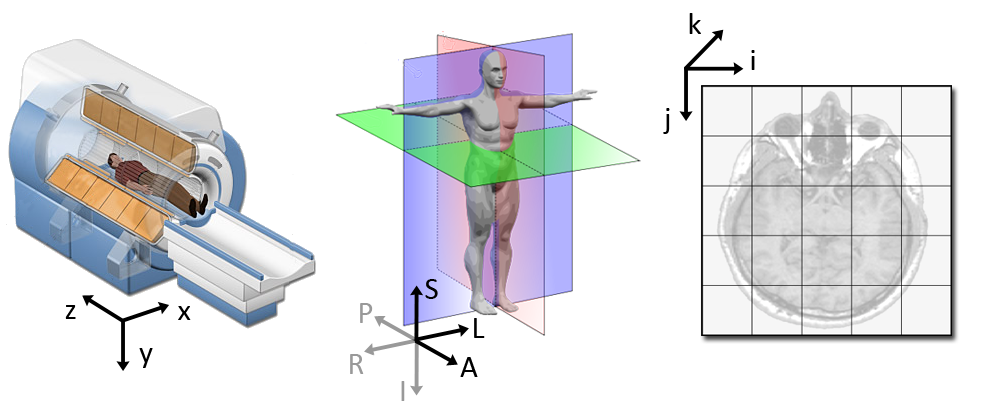
\includegraphics{Coordinate_sytems.png}
		\bicaption[CT扫描仪坐标系,人体坐标系和DICOM图像坐标系对应关系]
			{CT扫描仪坐标系,人体坐标系和DICOM图像坐标系对应关系\parencite{ctcoordinatesys2022, adaloglou2020dicomcoordinates}}
			{CT scanner, human body and DICOM imaging coordinates}
		\label{fig:coordinate}
	\end{figure}
	这样,分割出来的支气管气道树三维模型其每一个体素(Voxel)就具有精确的坐标位置信息,就可以计算出支气管管腔的中心线位置。
	
	导管机器人就是沿着管腔中心线的路径移动,导航至靶标位置。目前,美国Intuitive Surgical Company已经开发出肺部导管机器人ION,并投入了临床应用。
	\begin{figure}[!htp]
		\centering
		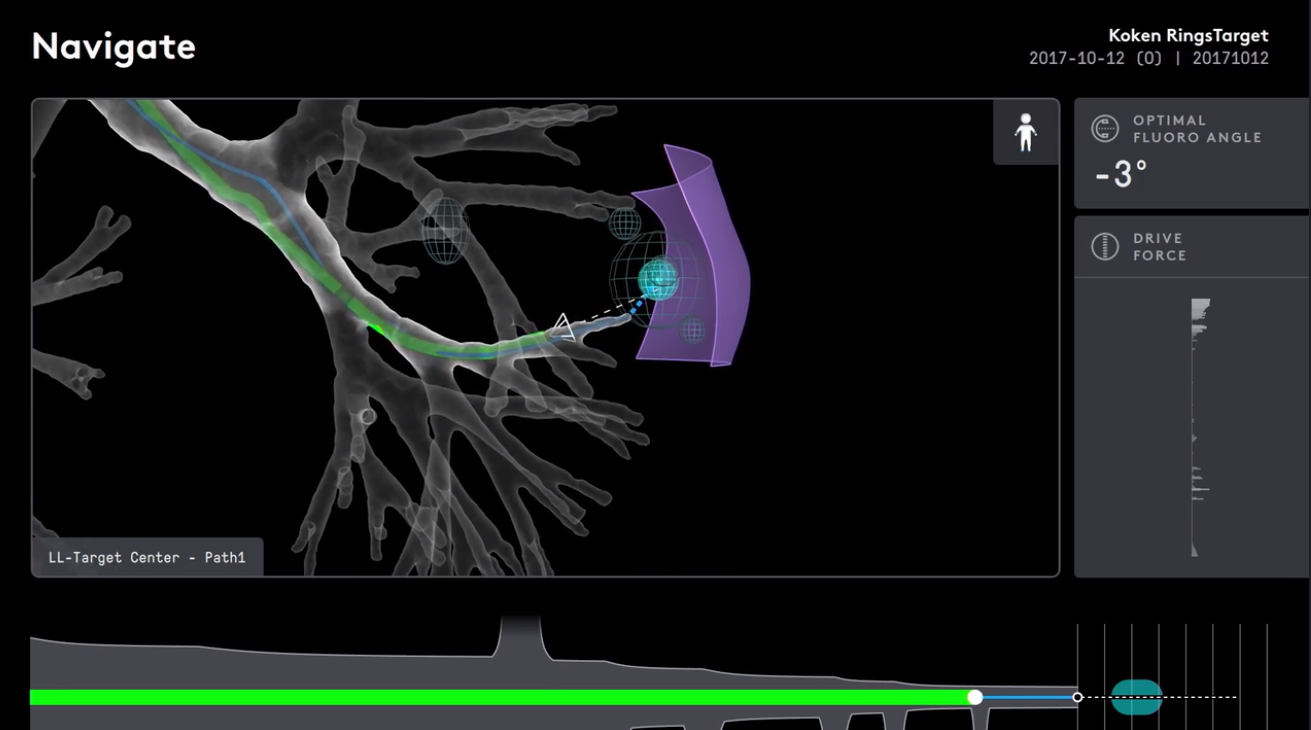
\includegraphics[width=0.45 \textwidth]{ION_robot_navigating}
		\hspace{2mm}
		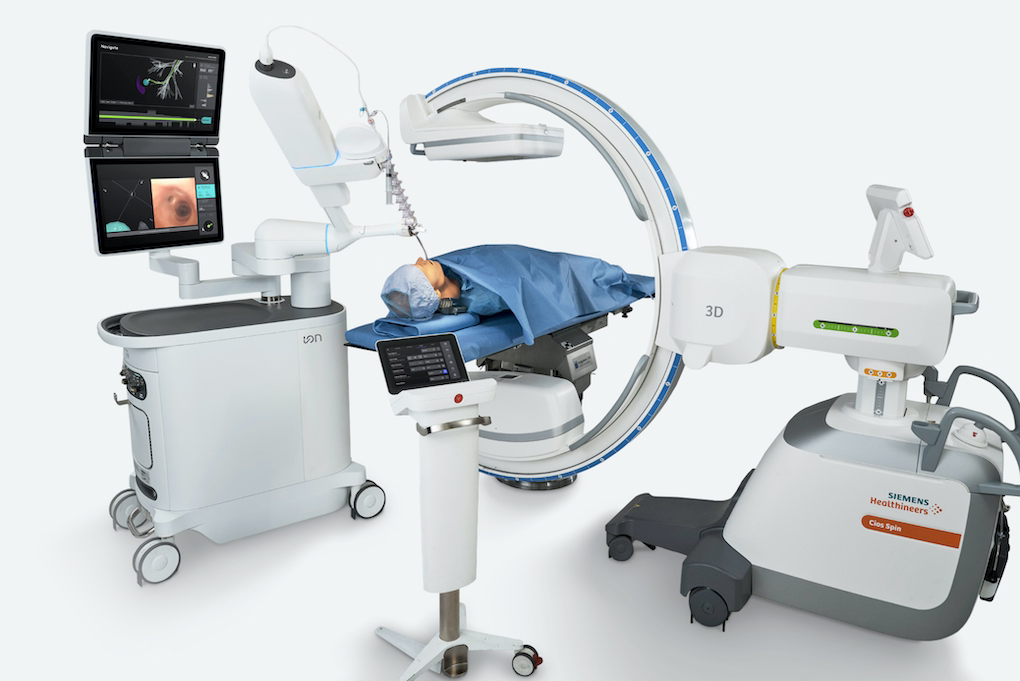
\includegraphics[width=0.45 \textwidth]{ION_bronchoscopy_robot.jpg}
		\bicaption[ION肺部导管机器人]
			{ION肺部导管机器人\parencite{ionrobot2021}}
			{ION bronchoscopy robot}
		\label{fig:ION_robot}
	\end{figure}
	
	作者所在的工作单位正在开发国产的肺部导管机器人,已经完成全国首例机器人辅助经支气管镜肺结节活检手术。
	
	当然导管手术机器人除了依赖支气管气道树三维模型导航,还需要辅助术中实时定位、支气管镜视觉导航的技术。
	
	
	\item {\heiti 智慧医疗辅助诊断}
	基于CT扫描图像的医疗图像分割需要高质量的标注数据,这很大程度上依赖经验丰富的临床医生/专家的专业知识。 为了减轻临床医生的标注压力和负担,同时亦为了减少误诊和漏诊
	的情况发生,医疗图像分割技术在医学辅助诊断上已经获得越来越多的应用。 具体到支气管气道树分割技术上,已经被用来辅助诊断一些慢性阻塞性肺部疾病COPD, 支气管扩张和肺气肿
	等一些肺部疾病。 随着AI图像分割技术的不断的进步,可以辅助临床医生更准确更高效地诊断疾病,逐渐达成智慧医疗,提高医疗技术水平和能力。
\end{itemize}



\section{研究现状和发展趋势}





\chapter{简介}

这是 \sjtuthesis 的示例文档,基本上覆盖了模板中所有格式的设置。建议大家在使用模
板之前,除了阅读《\sjtuthesis\ 使用文档》,这个示例文档也最好能看一看。

\section{二级标题}

\subsection{三级标题}

\subsubsection{四级标题}

Lorem ipsum dolor sit amet, consectetur adipiscing elit, sed do eiusmod tempor
incididunt ut labore et dolore magna aliqua. Ut enim ad minim veniam, quis
nostrud exercitation ullamco laboris nisi ut aliquip ex ea commodo consequat.
Duis aute irure dolor in reprehenderit in voluptate velit esse cillum dolore eu
fugiat nulla pariatur. Excepteur sint occaecat cupidatat non proident, sunt in
culpa qui officia deserunt mollit anim id est laborum.

\section{脚注}

Lorem ipsum dolor sit amet, consectetur adipiscing elit, sed do eiusmod tempor
incididunt ut labore et dolore magna aliqua. \footnote{Ut enim ad minim veniam,
quis nostrud exercitation ullamco laboris nisi ut aliquip ex ea commodo
consequat. Duis aute irure dolor in reprehenderit in voluptate velit esse cillum
dolore eu fugiat nulla pariatur.}

\section{字体}


上海交通大学是我国历史最悠久的高等学府之一,是教育部直属、教育部与上海市共建的全
国重点大学,是国家“七五”、“八五”重点建设和“211 工程”、“985 工程”的首批建
设高校。经过 115 年的不懈努力,上海交通大学已经成为一所“综合性、研究型、国际化”
的国内一流、国际知名大学,并正在向世界一流大学稳步迈进。 

{\songti 十九世纪末,甲午战败,民族危难。中国近代著名实业家、教育家盛宣怀和一批
  有识之士秉持“自强首在储才,储才必先兴学”的信念,于 1896 年在上海创办了交通大
  学的前身——南洋公学。建校伊始,学校即坚持“求实学,务实业”的宗旨,以培养“第
  一等人才”为教育目标,精勤进取,笃行不倦,在二十世纪二三十年代已成为国内著名的
  高等学府,被誉为“东方MIT”。抗战时期,广大师生历尽艰难,移转租界,内迁重庆,
  坚持办学,不少学生投笔从戎,浴血沙场。解放前夕,广大师生积极投身民主革命,学校
  被誉为“民主堡垒”。}

{\heiti 新中国成立初期,为配合国家经济建设的需要,学校调整出相当一部分优势专业、
  师资设备,支持国内兄弟院校的发展。五十年代中期,学校又响应国家建设大西北的号
  召,根据国务院决定,部分迁往西安,分为交通大学上海部分和西安部分。1959 年 3月
  两部分同时被列为全国重点大学,7 月经国务院批准分别独立建制,交通大学上海部分启
  用“上海交通大学”校名。历经西迁、两地办学、独立办学等变迁,为构建新中国的高等
  教育体系,促进社会主义建设做出了重要贡献。六七十年代,学校先后归属国防科工委和
  六机部领导,积极投身国防人才培养和国防科研,为“两弹一星”和国防现代化做出了
  巨大贡献。}

{\kaishu 改革开放以来,学校以“敢为天下先”的精神,大胆推进改革:率先组成教授代
  表团访问美国,率先实行校内管理体制改革,率先接受海外友人巨资捐赠等,有力地推动
  了学校的教学科研改革。1984 年,邓小平同志亲切接见了学校领导和师生代表,对学校
  的各项改革给予了充分肯定。在国家和上海市的大力支持下,学校以“上水平、创一流”
  为目标,以学科建设为龙头,先后恢复和兴建了理科、管理学科、生命学科、法学和人文
  学科等。1999 年,上海农学院并入;2005 年,与上海第二医科大学强强合并。至此,学
  校完成了综合性大学的学科布局。近年来,通过国家“985 工程”和“211 工程”的建
  设,学校高层次人才日渐汇聚,科研实力快速提升,实现了向研究型大学的转变。与此同
  时,学校通过与美国密西根大学等世界一流大学的合作办学,实施国际化战略取得重要突
  破。1985 年开始闵行校区建设,历经 20 多年,已基本建设成设施完善,环境优美的现
  代化大学校园,并已完成了办学重心向闵行校区的转移。学校现有徐汇、闵行、法华、七
  宝和重庆南路(卢湾)5 个校区,总占地面积 4840 亩。通过一系列的改革和建设,学校
  的各项办学指标大幅度上升,实现了跨越式发展,整体实力显著增强,为建设世界一流大
  学奠定了坚实的基础。}

{\ifcsname fangsong\endcsname\fangsong\else[无 \cs{fangsong} 字体。]\fi 交通大学
  始终把人才培养作为办学的根本任务。一百多年来,学校为国家和社会培养了 20余万各
  类优秀人才,包括一批杰出的政治家、科学家、社会活动家、实业家、工程技术专家和医
  学专家,如江泽民、陆定一、丁关根、汪道涵、钱学森、吴文俊、徐光宪、张光斗、黄炎
  培、邵力子、李叔同、蔡锷、邹韬奋、陈敏章、王振义、陈竺等。在中国科学院、中国工
  程院院士中,有 200 余位交大校友;在国家 23 位“两弹一星”功臣中,有 6 位交大校
  友;在 18 位国家最高科学技术奖获得者中,有 3 位来自交大。交大创造了中国近现代
  发展史上的诸多“第一”:中国最早的内燃机、最早的电机、最早的中文打字机等;新中国
  第一艘万吨轮、第一艘核潜艇、第一艘气垫船、第一艘水翼艇、自主设计的第一代战斗
  机、第一枚运载火箭、第一颗人造卫星、第一例心脏二尖瓣分离术、第一例成功移植同种
  原位肝手术、第一例成功抢救大面积烧伤病人手术等,都凝聚着交大师生和校友的心血智
  慧。改革开放以来,一批年轻的校友已在世界各地、各行各业崭露头角。}

{\ifcsname lishu\endcsname\lishu\else[无 \cs{lishu} 字体。]\fi 截至 2011 年 12
  月 31 日,学校共有 24 个学院 / 直属系(另有继续教育学院、技术学院和国际教育学
  院),19 个直属单位,12 家附属医院,全日制本科生 16802 人、研究生24495 人(其
  中博士研究生 5059 人);有专任教师 2979 名,其中教授 835 名;中国科学院院士 15
  名,中国工程院院士 20 名,中组部“千人计划”49 名,“长江学者”95 名,国家杰出
  青年基金获得者 80 名,国家重点基础研究发展计划(973 计划)首席科学家 24名,国
  家重大科学研究计划首席科学家 9名,国家基金委创新研究群体 6 个,教育部创新团队
  17 个。}

{\ifcsname youyuan\endcsname\youyuan\else[无 \cs{youyuan} 字体。]\fi 学校现有本
  科专业 68 个,涵盖经济学、法学、文学、理学、工学、农学、医学、管理学和艺术等九
  个学科门类;拥有国家级教学及人才培养基地 7 个,国家级校外实践教育基地 5个,国
  家级实验教学示范中心 5 个,上海市实验教学示范中心 4 个;有国家级教学团队 8个,
  上海市教学团队 15 个;有国家级教学名师 7 人,上海市教学名师 35 人;有国家级精
  品课程 46 门,上海市精品课程 117 门;有国家级双语示范课程 7 门;2001、2005 和
  2009 年,作为第一完成单位,共获得国家级教学成果 37 项、上海市教学成果 157
  项。}
